
\chapter{Views and templates}

\section{Overview}

A view is a ``type'' of Web page in your Django application that generally serves a specific function and has a specific template. 

In Django, web pages and other content are delivered by views.
Each view is represented by a Python function (or method, in the case of class-based views).
Django will choose a view by examining the URL that’s requested (to be precise, the part of the URL after the domain name).

To get from a URL to a view, Django uses what are known as 'URLconfs'.
A URLconf maps URL patterns to views.


\section{Writing more views}

Let's add a few more views to \keyword{polls/views.py}.
\lstset{language=Python}
\begin{lstlisting}
from django.shortcuts import render
from django.http import HttpResponse


# Create your views here.
def index(request):
    return HttpResponse("Hello, world. You're at the polls index.")


def detail(request, question_id):
    return HttpResponse("You're looking at question %s." % question_id)


def results(request, question_id):
    response = "You're looking at the results of question %s."
    return HttpResponse(response % question_id)


def vote(request, question_id):
    return HttpResponse("You're voting on question %s." % question_id)
  
\end{lstlisting}


Wire these new views into the \keyword{polls.urls} module by adding the following \keyword{path()} calls:
\begin{lstlisting}
from django.urls import path
from . import views

urlpatterns = [
    path('', views.index, name='index'),
    path('<int:question_id>/', views.detail, name='detail'),
    path('<int:question_id>/results/', views.results, name='results'),
    path('<int:question_id>/votes/', views.vote, name='vote')
]
\end{lstlisting}


Visite the website \url{localhost:8000/polls/1/} or \url{localhost:8000/polls/1/results} or \url{localhost:8000/polls/1/votes}, you will get the corresponding view.

See Figure \ref{fig:view}:
\begin{figure}[!ht]
  \centering
  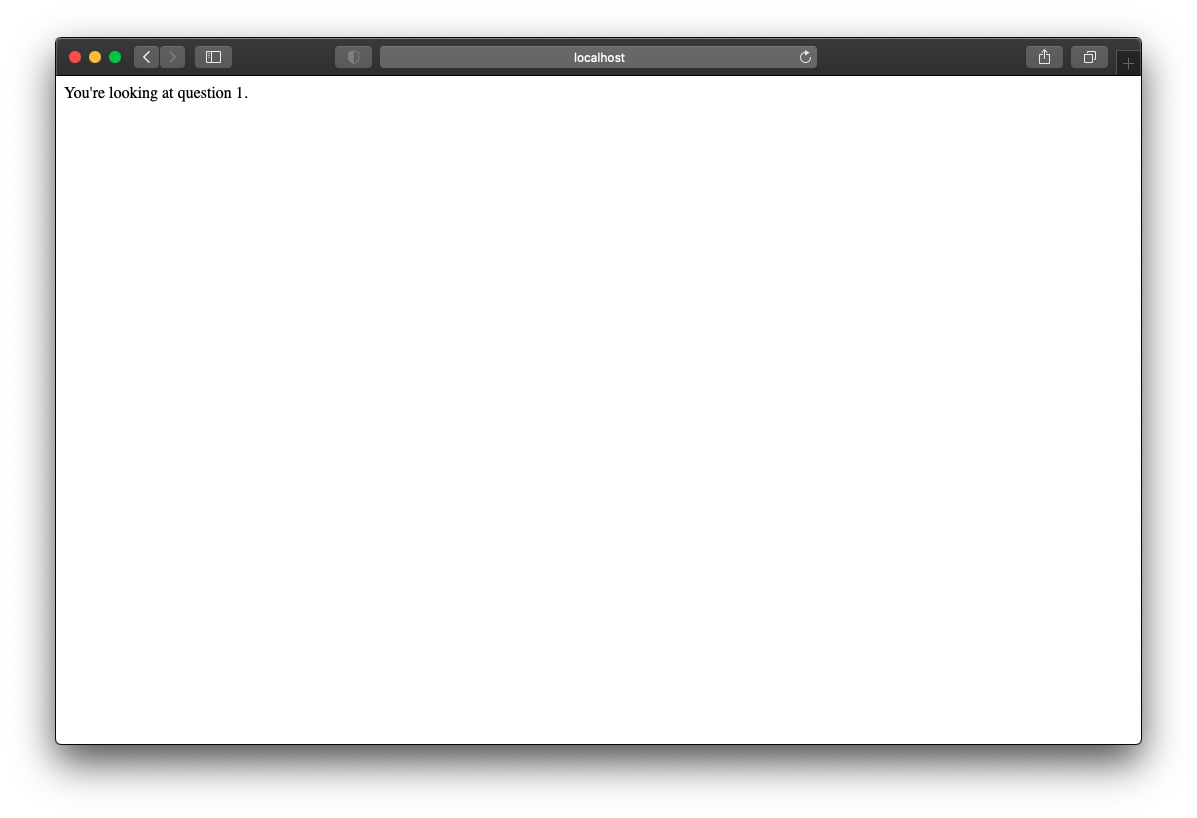
\includegraphics[width=\textwidth]{view.png}
  \caption{View}
  \label{fig:view}
\end{figure}


\section{Write views that actually do something}

Each view is responsible for doing one of two things: returning an \keyword{HttpResponse} object containing the content for the requested page, or raising an exception such as \keyword{Http404}.
The rest is up to you.


\begin{lstlisting}
def index(request):
    # return HttpResponse("Hello, world. You're at the polls index.")
    latest_question_list = Question.objects.order_by('-pub_date')[:5]
    output = ', '.join([q.question_text for q in latest_question_list])
    return HttpResponse(output)
\end{lstlisting}

There’s a problem here, though: the page’s design is hard-coded in the view.
If you want to change the way the page looks, you’ll have to edit this Python code.
So let’s use Django’s template system to separate the design from Python by creating a template that the view can use.

The structure is shown in Figure \ref{fig:templates}:
\begin{figure}[!ht]
  \centering
  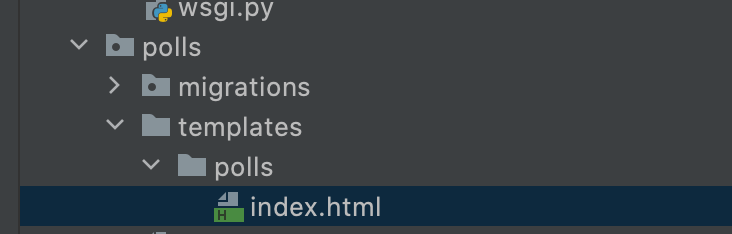
\includegraphics[width=\textwidth]{templates.png}
  \caption{Templates}
  \label{fig:templates}
\end{figure}


\begin{lstlisting}
from django.shortcuts import render

from .models import Question


def index(request):
    latest_question_list = Question.objects.order_by('-pub_date')[:5]
    context = {'latest_question_list': latest_question_list}
    return render(request, 'polls/index.html', context)
\end{lstlisting}


\section{Raising a 404 error}
polls/views.py:
\begin{lstlisting}
from django.shortcuts import get_object_or_404, render

from .models import Question
# ...
def detail(request, question_id):
    question = get_object_or_404(Question, pk=question_id)
    return render(request, 'polls/detail.html', {'question': question})
  \end{lstlisting}


polls/templates/polls/detail.html:
\begin{verbatim}
{{ question }}
\end{verbatim}
  

\section{Use the template system}

polls/templates/polls/detail.html:
\begin{verbatim}
<h1>{{ question.question_text }}</h1>
<ul>

    <li>{{ choice.choice_text }}</li>

</ul>
\end{verbatim}

\section{Removing hardcoded URLs in templates}

From:
\begin{lstlisting}
<li><a href="/polls/{{ question.id }}/">{{ question.question_text }}</a></li>
\end{lstlisting}

To:
\begin{lstlisting}
<li><a href="">{{ question.question_text }}</a></li>
\end{lstlisting}

\section{Namespacing URL names}

polls/urls.py:
\begin{lstlisting}
app_name = 'polls'
\end{lstlisting}

To:
\begin{lstlisting}
<li><a href="">{{ question.question_text }}</a></li>  
\end{lstlisting}


